%-------------------------------------STYLES----------------------------------------------------------------%

\documentclass[10pt, xcolor=dvipsnames]{beamer}

%\mode<presentation>
%{
\usetheme{Madrid}
%\setbeamercovered{transparent}
%} 
%\usefonttheme{professionalfonts}
\usecolortheme{seahorse}

\usepackage{setspace}
\usepackage[english]{babel}
\usepackage[latin1]{inputenc}
\usepackage{times}
\usepackage[T1]{fontenc}
\usepackage{color}
\usepackage{graphicx}
\usepackage{amssymb}
\usepackage{amsthm}
\usepackage{bm}
\usepackage{rotating}
\usepackage{ccaption}
\usepackage{booktabs}
\usepackage{lscape}
\usepackage{colortbl}
\usepackage{arydshln}
\usepackage{tabularx}

%\useinnertheme{rounded}
\setbeamertemplate{items}[balls]
%\usepackage[notocbib]{apacite}                % This is bibliography package.
%\renewcommand{\bibliographytypesize}{\tiny}
\setbeamertemplate{navigation symbols}{}
\usepackage{graphics}
\usepackage{epstopdf}
\DeclareGraphicsRule{.tif}{png}{.png}{`convert #1 `dirname #1`/`basename #1 .tif`.png}
%\usepackage{fleqn}
%\setlength{\mathindent}{1cm}
%\color{white}
%\hypersetup{colorlinks=true,linkcolor=Blue}
\usepackage{bbm}
\newcommand{\backupbegin}{
   \newcounter{framenumberappendix}
   \setcounter{framenumberappendix}{\value{framenumber}}
}
\newcommand{\backupend}{
   \addtocounter{framenumberappendix}{-\value{framenumber}}
   \addtocounter{framenumber}{\value{framenumberappendix}}
}

%% Change the margins
\newenvironment{changemargin}[2]{%
  \begin{list}{}{%
    \setlength{\topsep}{0pt}%
    \setlength{\leftmargin}{#1}%
    \setlength{\rightmargin}{#2}%
    \setlength{\listparindent}{\parindent}%
    \setlength{\itemindent}{\parindent}%
    \setlength{\parsep}{\parskip}%
  }%
  \item[]}{\end{list}}


%-------------------------------------------Title---------------------------------------------------%


\title[Land Constraints]{{How Tight are Malthusian Constraints?}}

\author[Johnson \& Vollrath]{T. Ryan Johnson \inst{1} \and Dietrich Vollrath \inst{2}}
\institute[UH]{\inst{1} University of Houston \and %
                      \inst{2} University of Houston}

\date[February 2017]{}

%-------------------------------------------Slides---------------------------------------------------%

\begin{document}
\maketitle

\section{Introduction}


\begin{frame}{The Historical Relevance of Malthus}
 
 ``\textit{But the logic of the Malthusian model matches the empirical evidence for the preindustrial world. While even long before the Industrial Revolution small elites had an opulent lifestyle, the average person in 1800 was no better off than his or her ancestors of the Paleolithic or Neolithic.}'' - Clark (2007)

\vspace{1cm}
 ``\textit{During the Malthusian Epoch....technologically superior countries eventually developed denser populations, but their standards of living did not reflect the degree of their technological advancements.}'' - Galor (2011)

\end{frame}

\begin{frame}{Malthusian Pressures?}
``\textit{To the extent that it left such improvements to be realized in the future, eighteenth-century European farming left more room to continue growth before encountering Malthusian constraints than was present in east Asia.}'' - Pomeranz (2000)

\vspace{.5cm}
``\textit{Clearly the shortage of many resources grew more severe [in China] ... A major cause of these shortages was of course the continuing growth of the population under conditions of relative technological standstill.}'' - Elvin (1973)

\vspace{.5cm}
``\textit{In both regions population grew over the period 1680 to 1850: In China from an estimated 150 million to an estimated 400-410 million and in Western Europe from some seventy-five million to some 170 million and in both there were Malthusian pressures.}'' - Vries (2013)
\end{frame}

\begin{frame}{The Continued Relevance of Malthus}
``\textit{[Africa's] countries remain mired in a Malthusian crisis of high mortality, high fertility, and rapid population growth (with an accompanying state of chronic extreme poverty)}'' - Conley, McCord, and Sachs (2007)

\vspace{.5cm}
``\textit{The Malthusian channel by which a high level of population reduces income per capita is still relevant in poor developing countries that have large rural populations dependent on agriculture, as well as in countries that are heavily reliant on mineral or energy exports.}'' - Weil and Wilde (2009)

\vspace{.5cm}
``\textit{Our general aim is to build a theory of economy-environment interactions capable of addressing one of the main future challenges ... how to sustain innovation-driven income per capita growth in a habitat that has a finite carrying capacity of people.}'' - Peretto and Valente (2015)
\end{frame}


\begin{frame}{Malthusian?}
Some examples of usage:
\begin{itemize}
\item ``Malthusian constraints''
\item ``Malthusian pressure''
\item ``Malthusian limits''
\item ``Malthusian crisis''
\item ``Malthusian conditions binding''
\end{itemize}

\vspace{.5cm} What do we mean by a ``Malthusian constraint''? 
\end{frame}

\begin{frame}{Definition}\label{define}
For us: the Malthusian constraint is the \textit{elasticity of output with respect to agricultural land}. 

\vspace{.2cm} This answers:
\begin{itemize}
\item How important is land to production?
\item How does the average product of labor change with respect to labor?
\item How sensitive is economy to a \textit{change} in population?
\end{itemize}

\hfill \hyperlink{toy}{\beamerbutton{Toy Model}}
\end{frame}

\begin{frame}{Basic idea}
Look at relationship of density and inherent agricultural produtivity (TFP)
\begin{itemize}
  \item If density is sensitive to productivity $\Rightarrow$ \textit{loose} Malthusian constraint
  \item If density is insensitive to productivity $\Rightarrow$ \textit{tight} Malthusian constraint
\end{itemize}

\end{frame}

\begin{frame}{Density and Productivity, by Region, 1500CE}
\begin{center}
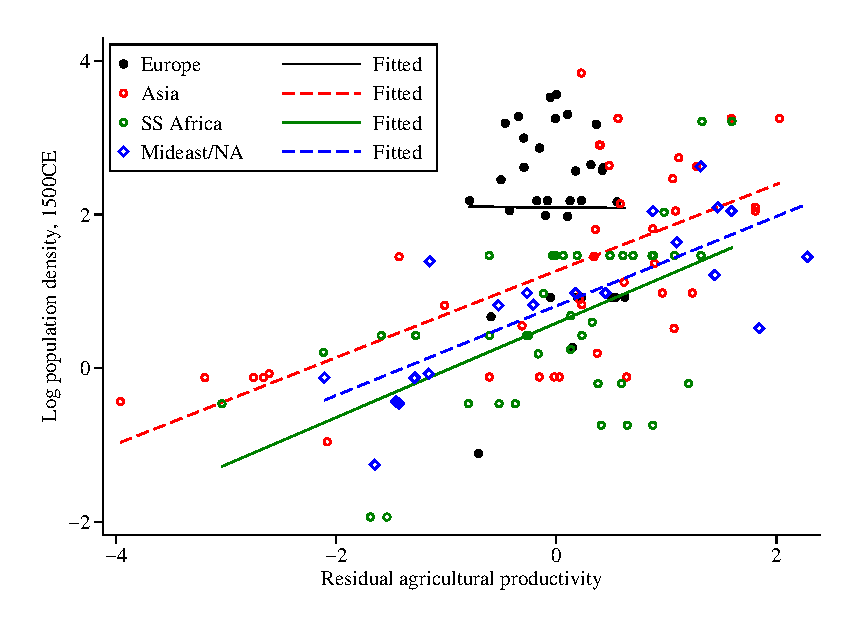
\includegraphics[width=.8\textwidth]{fig_ag_regions.eps}
\end{center}
{\scriptsize Data from Ashraf and Galor (2010). Residual plot using their controls except continent FE.}
\end{frame}


\begin{frame}{In this paper}
Estimate the Malthusian constraint:
\begin{itemize}
  \item Use relationship of \textit{rural} density and agro-climatic agricultural TFP
  \item Estimates come from \textit{within}-province variation (province FE)
  \item Population data from HYDE
  \item Agro-climatic TFP built from Galor and {\"O}zak data on caloric suitability
\end{itemize}

\vspace{.2cm} We find:
\begin{itemize}
  \item Constraints range from 0.090 to 0.308
  \item Variation is related to agro-climatic conditions
  \item Temperate, cold, regular rain $\Rightarrow$ tight Malthusian constraints
  \item Equatorial, hot, seasonal rain $\Rightarrow$ loose Malthusian constraints
\end{itemize}

\end{frame}

\begin{frame}{Implications}
Pattern of results:
\begin{itemize}
  \item No strict relationship with development
  \item Rich places today do not (did not?) have looser Malthusian constraints
\end{itemize}

\vspace{.2cm} But..
\begin{itemize}
  \item Constraint determines how sensitive real wages and agric. labor share are to shocks
  \item Tight constraint $\Rightarrow$ very sensitive (and v.v.)
\end{itemize}

\vspace{.2cm} So says something about role of following in development:
\begin{itemize}
  \item Population shocks (epidemics, mortality transition)
  \item Affect response to technology shocks (new crops or better crops)
\end{itemize}

\end{frame}


\begin{frame}{Some Related Literature:}
\begin{itemize}
  \item \textbf{Geography and development:} Olsson and Hibbs (2005); Ashraf and Galor (2011); Nunn and Qian (2011); Nunn and Puga (2012); Michalopoulos (2012); Alesina, Giuliano, Nunn (2013); Cook (2014a,b); Fenske (2014); Alsan (2015); Ashraf and Michalopoulos (2015); Dalgaard, Knudsen, Selaya (2015); Galor and {\"O}zak (2016); Litina (2016); Andersen, Dalgaard, Selaya (2016); Frankema and Papaioannou (2017)
  \item \textbf{Malthusian and UGT models:} Galor (2011); Galor and Weil (2000); Galor and Moav (2002); Hansen and Prescott (2002); Doepke (2004); Cervellati and Sunde (2005); L{\"a}gerlof (2006); Crafts and Mills (2009); Strulik and Weisdorf (2008), Voigtl{\"a}nder and Voth (2013a,b)
  \item \textbf{Agriculture and development:} Gollin, Parente, Rogerson (2007); Restuccia, Yang, Zhu (2008); Weil and Wilde (2009), Gollin (2010)
\end{itemize}

\vspace{.2cm} Two specific:
\begin{itemize}
  \item Motamed, Florax, Master (2014): Pattern/date of urbanization at grid-cell level based on agro-climatic conditions
  \item Henderson, Squires, Storeygard, Weil (2016): Spatial organization of economic activity, relationship to geograhpic conditions
\end{itemize}

\end{frame}

\section{Model}

\begin{frame}{A Model of Density and Productivity}
Region $I$ contains a set of districts, each denoted by $i$, with aggregate agricultural production
\begin{equation}
Y_{i} = A_{i} X_{i}^{\beta} \left(K_{Ai}^{\alpha}L_{Ai}^{1-\alpha}\right)^{1-\beta} \label{EQ_production}
\end{equation}
\begin{itemize}
  \item $K_{Ai}$ is all other inputs (e.g. capital)
  \item $L_{Ai}$ is agricultural labor in district $i$ (not a single sector)
  \item Assume $\beta$ and $\alpha$ are identical \textit{within} region (but not nec. \textit{across} regions)
  \item Elasticity of $Y_i/L_{Ai}$ w.r.t. $L_{Ai}$ is $\alpha + \beta(1-\alpha)$
\end{itemize}
\end{frame}

\begin{frame}{Mobile Factors}
The wage and return to capital in each district are given by 
\begin{eqnarray}
    w = \phi_L \frac{Y_i}{L_i} \\ \nonumber
    r = \phi_K \frac{Y_i}{K_i} \label{EQ_factorprices}
\end{eqnarray}
\begin{itemize}
  \item $\phi_L$ and $\phi_K$ are shares of output 
  \item No assumption that shares = elasticities
  \item Shares are identical \textit{within} region (but not nec. \textit{across} regions)
  \item Capital and labor are mobile \textit{within} region (but not nec. \textit{across} regions)
\end{itemize}
\end{frame}

\begin{frame}{Solving for Labor Allocations}
Given mobility of labor and capital within region,
\begin{equation}
    \frac{K_i}{L_{Ai}} = \frac{w}{r}\frac{\phi_K}{\phi_L}.
\end{equation}
Adding up condition for agricultural labor within region
\begin{equation}
\sum_{i\in I} L_{Ai} = L_A.
\end{equation}
Solve for allocation of labor (relative to land) to district $i$
\begin{equation}
\frac{L_{Ai}}{X_i} = A_{i}^{1/\beta}\frac{L_A}{\sum_{j\in I} A_{j}^{1/\beta}X_{j}}. \label{EQ_LaX}
\end{equation}
\end{frame}

\begin{frame}{Agricultural Labor Allocation}
Take logs of $L_{Ai}/X_i$ expression
\begin{equation}
\ln L_{Ai}/X_i = \frac{1}{\beta} \ln A_{i} + \ln \Gamma, \label{EQ_est}
\end{equation}
where
\begin{equation}
    \Gamma = \frac{L_A}{\sum_{j\in I} A_{j}^{1/\beta}X_{j}}.
\end{equation}
is a \textit{region-specific} term. 

\begin{itemize}
  \item $\beta$ can be estimated from elasticity of $L_{Ai}/X_i$ w.r.t. $A_i$. 
  \item $1/\beta$ small (tight), ag. workers spread evenly w/in region
  \item $1/\beta$ large (loose), ag. workers concentrated on high $A_i$
\end{itemize}
\end{frame}

\begin{frame}{Agricultural Labor Allocation}
Take logs $L_{Ai}/X_i$ expression
\begin{equation}
\ln L_{Ai}/X_i = \frac{1}{\beta} \ln A_{i} + \ln \Gamma, \label{EQ_est}
\end{equation}
where
\begin{equation}
    \Gamma = \frac{L_A}{\sum_{j\in I} A_{j}^{1/\beta}X_{j}}.
\end{equation}
is a \textit{region-specific} term. 

\begin{itemize}
  \item $\Gamma$ is constant for all districts w/in region
  \item Ag labor relative to total labor ($L_A/L$) does not affect $\beta$ or $\Gamma$
  \item Expression is not unique to heaviliy agricultural regions (or eras)
\end{itemize}
\end{frame}

\section{Regression Setup}

\begin{frame}{Using as a Specification}
Re-arranging the prior expression and adding some notation:
\begin{equation}
  \ln A_{isc} = \alpha + \beta \ln L_{Aisc}/X_{isc} + \gamma_{sc} + \delta' \mathbf{Z}_{isc} + \epsilon_{isc}. \label{EQ_regress}
\end{equation}

\begin{itemize}
  \item District $i$, region/state/province $s$, country $c$
  \item $\gamma_{sc}$, region/country FE, pick up $\Gamma$ term
  \item $\mathbf{Z}_{isc}$ are additional controls
  \item $\epsilon_{isc}$ is error term
\end{itemize}
\end{frame}

\begin{frame}{Using as a Specification}
YES, we moved productivity, $A_{isc}$ and agric. density $L_{Aisc}/X_{isc}$ to opposite sides:
\begin{equation}
  \ln A_{isc} = \alpha + \beta \ln L_{Aisc}/X_{isc} + \gamma_{sc} + \delta' \mathbf{Z}_{isc} + \epsilon_{isc}. \label{EQ_regress}
\end{equation}

\begin{itemize}
  \item NO, This is NOT a causal statement
  \item Estimating $1/\beta$ is difficult as $\beta$ gets close to zero
\end{itemize}
\end{frame}

\begin{frame}{Agricultural Density Data}
$L_{Aisc}$ comes from HYDE 3.1 database (Goldewijk et al, 2011)
\begin{itemize}
  \item Population counts for 5 degree grid-cells built from administrative data
  \item We aggregate data back to administrative level (e.g. districts)
  \item (In progress) Validating against administrative data
  \item Rural population data (not agricultural)
  \item Main samples based on year 2000
\end{itemize}
$X_{isc}$ calculated as area of a given district
\begin{itemize}
  \item Overstates size of agricultural land
\end{itemize}
$L_{Aisc}/X_{isc}$ data 
\begin{itemize}
  \item Trim above 99th and below 1st percentiles
  \item Drop if fewer than 100 total rural residents
  \item 29,030 total districts
\end{itemize}
\end{frame}

\begin{frame}{Agricultural Density Data}
\begin{center}
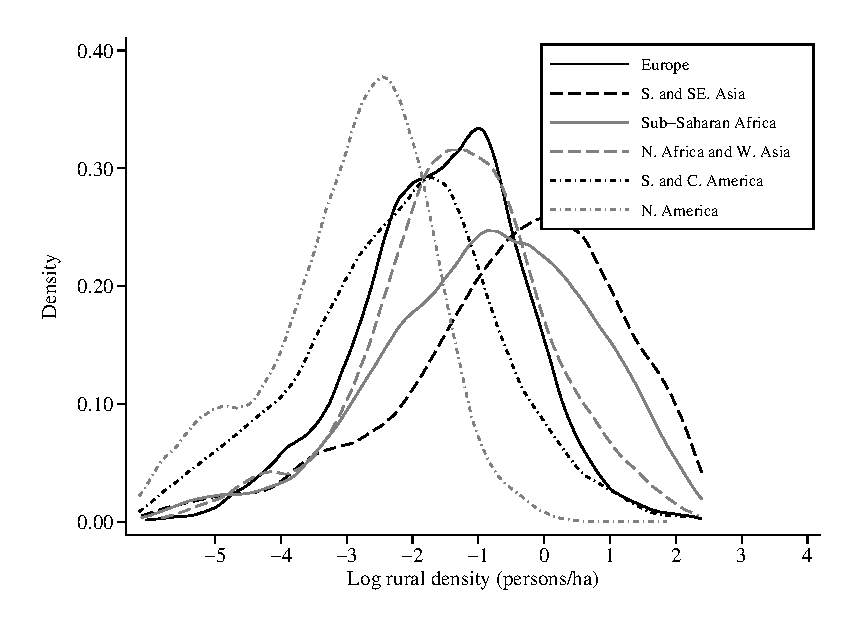
\includegraphics[width=.8\textwidth]{fig_dens_rurd.eps}
\end{center}
\end{frame}

\begin{frame}{Agricultural Productivity Data}
$A_{isc}$ is built similar to Galor and {\"O}zak (2016) caloric suitability index
\begin{itemize}
  \item Data from GAEZ on agro-climatic possible yield (in raw tons) for each crop
  \item Combine with nutritional information by crop (total calories per raw ton)
  \item For each grid cell, determine max calories
  \item Total max calories across grid cells in district, divide by total area
  \item As in Galor and {\"O}zak, yield is holding technology constant
  \item Trim above 99th and below 1st percentile
\end{itemize}
\end{frame}

\begin{frame}{Agricultural Productivity Data}
\begin{center}
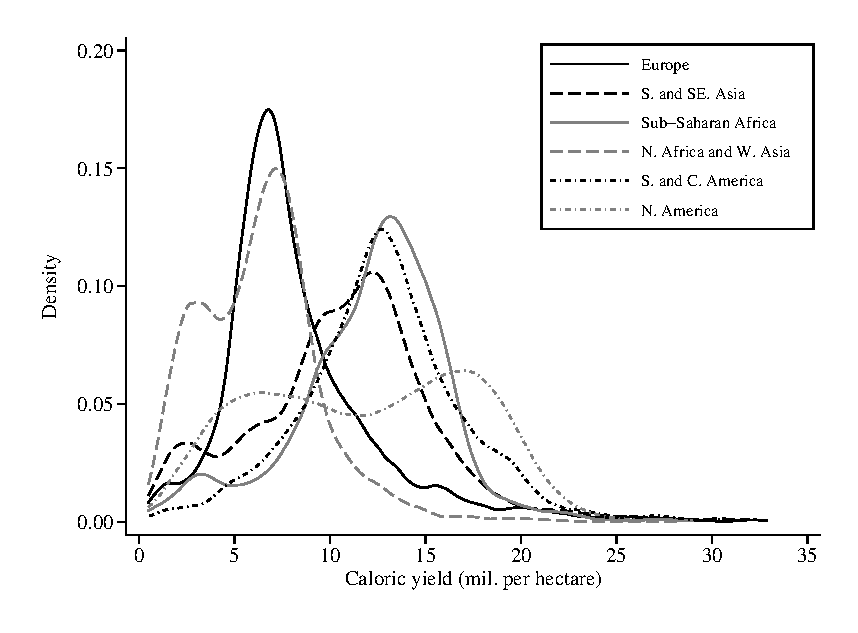
\includegraphics[width=.8\textwidth]{fig_dens_csi.eps}
\end{center}
\end{frame}

\begin{frame}{Agricultural Productivity Data}

\end{frame}

\begin{frame}{Control Variables}
Henderson et al (2016) on spatial distribution of economic activity
\begin{itemize}
  \item Urban activity correlated with (caused by?) high agricultural productivity (in some places)
  \item Low rural density because of urban activity
  \item $Corr(\epsilon_{isc},\ln L_{isc}/X_{isc})<0$
\end{itemize}

Include two controls at the district level in $\mathbf{Z}_{isc}$ for urban/economic activity:
\begin{itemize}
  \item Night lights density: follows Henderson et al (2016) using Global Radiance Calibrated data
  \item Urban percent of population: from HYDE
\end{itemize}

\end{frame}

\begin{frame}{Spatial Errors and Hypothesis Testing}\label{testing}
Assume $\epsilon_{isc}$ has spatial auto-correlation. Use Conley s.e. (1000km window). 

\vspace{.2cm} Two hypothesis tests:
\begin{itemize}
  \item Is the land constraint binding? 
    \begin{itemize}
      \item $H_0: \beta=0$ vs. two-sided alt 
    \end{itemize}
  \item Is the land constraint the same in two samples (e.g. Europe and Sub-Saharan Africa)? 
    \begin{itemize}
      \item $H_0: \beta = \beta^{Ref}$ vs. two-sided alt 
      \item $\beta^{Ref}$ from ad hoc ``reference'' sample
      \item Implemented with interaction regression combining given and reference sample
      \item In practice, choice of reference sample won't be crucial
    \end{itemize}
\end{itemize}
\hfill \hyperlink{interaction}{\beamerbutton{Interaction}}
\end{frame}

\section{Results}

\begin{frame}{Results by Major Region}
\begin{center}
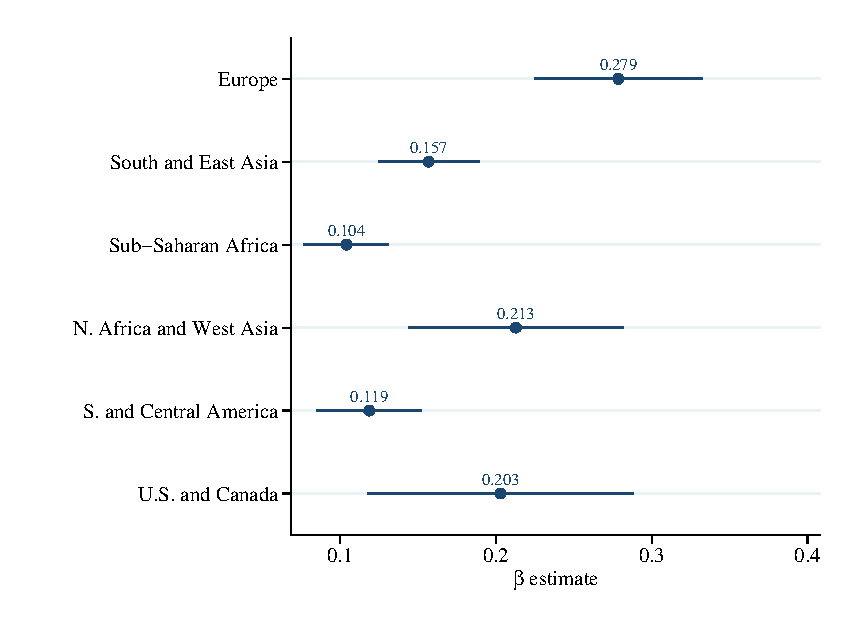
\includegraphics[width=.8\textwidth]{fig_coef_region.eps}
\end{center}
\end{frame}

\begin{frame}{Results by Major Region}

{\scriptsize
\begin{tabularx}{\textwidth}{lXXXXXX}
\midrule
\multicolumn{7}{l}{Dependent Variable: Log caloric yield ($A_{isc}$)} \\
 & \multicolumn{6}{c}{Region:} \\ \cmidrule{2-7}
 &        & East \& & Sub-        & North     & South \&  &  \\
 &        & South   & Saharan     & Africa \& & Central   & U.S. and \\
 & Europe & Asia    & Africa      & West Asia & America   & Canada \\
 & (1) & (2) & (3) & (4) & (5) & (6) \\
\midrule
Log rural density   &       0.279&       0.157&       0.104&       0.213&       0.119&       0.203\\
                    &     (0.027)&     (0.017)&     (0.014)&     (0.035)&     (0.017)&     (0.044)\\
\midrule
p-value $\beta=0$   &       0.000&       0.000&       0.000&       0.000&       0.000&       0.000\\
p-value $\beta=\beta^{Eur}$&           .&       0.000&       0.000&       0.137&       0.000&       0.142\\
Countries           &          34&          24&          43&          18&          25&           2\\
Observations        &        7514&        6761&        3210&        2762&        9131&        2782\\
Adjusted R-square   &        0.30&        0.24&        0.26&        0.28&        0.18&        0.28\\

\midrule
\end{tabularx}
}

\end{frame}

\begin{frame}{Results by Sub-Region}
\begin{center}
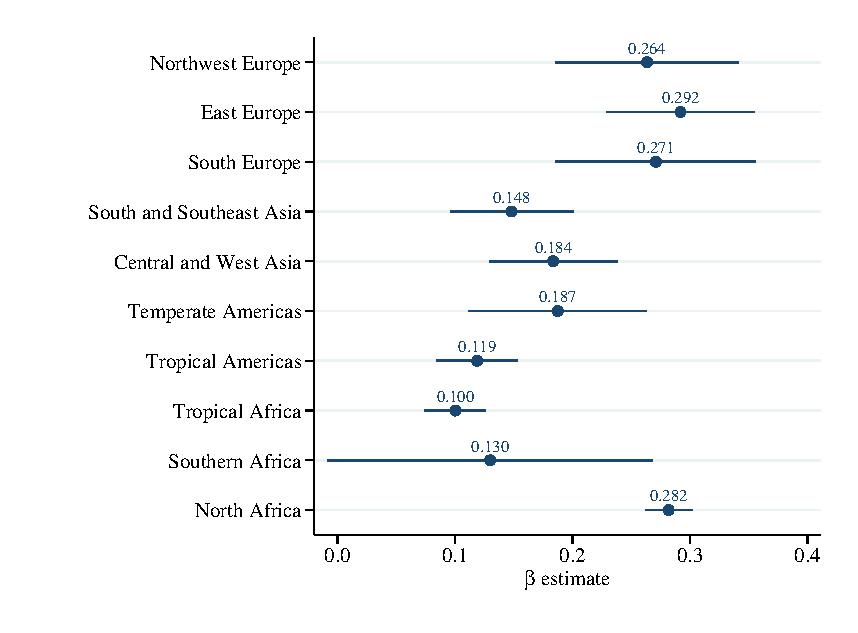
\includegraphics[width=.8\textwidth]{fig_coef_subregion.eps}
\end{center}
\end{frame}

\begin{frame}{Results by Sub-Region}

{\scriptsize
\begin{tabularx}{\textwidth}{lXXXXX}
\midrule
\multicolumn{6}{l}{Dependent Variable in both panels: Log caloric yield ($A_{isc}$)} \\ \\
\\
Panel A & \multicolumn{5}{c}{Sub-Region:} \\ \cmidrule{2-6}
 &          &         &             &  \multicolumn{2}{c}{Excl. China} \\ \cmidrule(lr){5-6}
 & North \& &         &              & South \&  & Central \&             \\
 & Western  & Eastern & Southern     & Southeast & West        \\
 & Europe   & Europe  & Europe       & Asia      & Asia      \\
 & (1) & (2) & (3) & (4) & (5) \\
\midrule
Log rural density   &       0.264&       0.292&       0.271&       0.148&       0.184\\
                    &     (0.040)&     (0.032)&     (0.043)&     (0.027)&     (0.028)\\
\midrule
p-value $\beta=0$   &       0.000&       0.000&       0.000&       0.000&       0.000\\
p-value $\beta=\beta^{NWEur}$&           .&       0.569&       0.884&       0.016&       0.099\\
Countries           &          16&           9&           9&          13&          18\\
Observations        &        1628&        4772&        1114&        3921&        2762\\
Adjusted R-square   &        0.21&        0.31&        0.26&        0.16&        0.18\\

\midrule
\end{tabularx}
}
\end{frame}

\begin{frame}{Results by Sub-Region}

{\scriptsize
\begin{tabularx}{\textwidth}{lXXXXX}
\midrule
\multicolumn{6}{l}{Dependent Variable in both panels: Log caloric yield ($A_{isc}$)} \\ \\
\\
Panel B & \multicolumn{5}{c}{Sub-Region:} \\ \cmidrule{2-6}
 &           &   &           &          &             \\
 & Temperate & Tropical  & Tropical & South    & North    \\
 & Americas  & Americas  & Africa   & Africa   & Africa     \\
\midrule
Log rural density   &       0.187&       0.119&       0.100&       0.130&       0.282\\
                    &     (0.039)&     (0.018)&     (0.013)&     (0.071)&     (0.010)\\
\midrule
p-value $\beta=0$   &       0.000&       0.000&       0.000&       0.066&       0.000\\
p-value $\beta=\beta^{NWEur}$&       0.170&       0.001&       0.000&       0.099&       0.654\\
Countries           &           5&          22&          39&           4&           5\\
Observations        &        3183&        8730&        3032&         178&        1147\\
Adjusted R-square   &        0.18&        0.10&        0.14&        0.19&        0.24\\

\midrule
\end{tabularx}
}

\end{frame}

\begin{frame}{Results for China, Japan, Korea}

{\scriptsize
\begin{tabularx}{\textwidth}{lXXXXX}
\midrule
\multicolumn{4}{l}{Dependent Variable: Log caloric yield ($A_{isc}$)} \\
 & All& Temperate & Sub-Trop & & N. \& \\
 & China & China  & China & Japan & S. Korea  \\
 & (1) & (2) & (3) & (4) & (5) \\
\midrule
Residuals           &       0.414&       0.518&       0.107&       0.155&       0.190\\
                    &     (0.089)&     (0.060)&     (0.021)&     (0.003)&     (0.060)\\
\midrule
p-value $\beta=0$   &       0.000&       0.000&       0.000&       0.000&       0.002\\
p-value $\beta=\beta^{Temp}$&            &            &       0.000&            &            \\
Observations        &         266&         130&         136&        1039&         311\\
Adjusted R-square   &        0.56&        0.70&        0.13&        0.23&        0.23\\

\midrule
\end{tabularx}
}

\end{frame}

\begin{frame}{Results by Province}
Regions and sub-regions assume $\beta$ constant within region/sub-region. Instead, estimate $\beta$ individually for each province
\begin{itemize}
  \item Only provinces with 6 or more districts (1,340 provinces)
  \item ... so really big SE on any individual estimate
  \item Look at pattern of $\beta$'s for each sub-region
\end{itemize}
\end{frame}

\begin{frame}{Results by Province}
\begin{center}
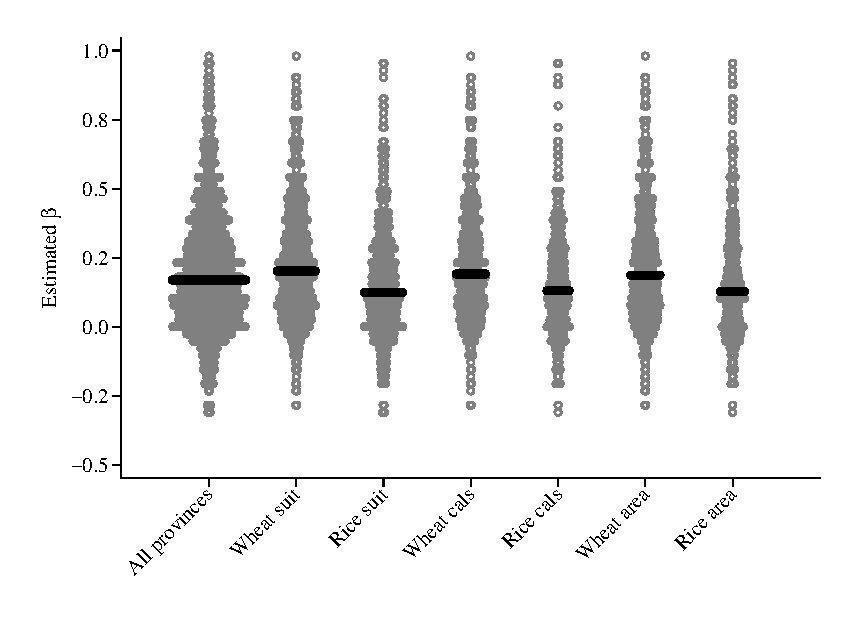
\includegraphics[width=.8\textwidth]{fig_beta_province.eps}
\end{center}
\end{frame}

\begin{frame}{Results by Province}

{\tiny
\begin{tabularx}{\textwidth}{lrXrXrXrXrXrXrXr}
\midrule
           &       &&      &&     && \multicolumn{9}{c}{Percentiles:} \\ \cmidrule{8-16}
Sub-region & Prov. && Mean && SD  && 10th    && 25th    && 50th && 75th && 90th \\
\midrule
All provinces &    1,183&     0.21&     0.23&    -0.02&     0.05&     0.18&     0.33&     0.49\\ \\
Wheat Suitable &      619&     0.23&     0.23&    -0.00&     0.08&     0.21&     0.36&     0.50\\
Rice Suitable &      469&     0.17&     0.24&    -0.04&     0.03&     0.15&     0.28&     0.43\\
Wheat cals>33\% &      457&     0.23&     0.22&    -0.00&     0.08&     0.21&     0.36&     0.50\\
Rice cals>33\% &      307&     0.18&     0.21&    -0.04&     0.03&     0.15&     0.29&     0.41\\
Wheat area>50\% &      485&     0.22&     0.23&    -0.01&     0.07&     0.20&     0.36&     0.53\\
Rice area>50\% &      297&     0.18&     0.23&    -0.04&     0.03&     0.14&     0.29&     0.47\\ \\
Northwest Europe &        79&     0.26&     0.31&     0.00&     0.08&     0.22&     0.46&     0.62\\
Eastern Europe &       173&     0.24&     0.20&     0.01&     0.09&     0.23&     0.38&     0.50\\
Southern Europe &        60&     0.27&     0.17&     0.08&     0.16&     0.25&     0.37&     0.50\\
South and S. East Asia &       248&     0.20&     0.23&    -0.03&     0.04&     0.16&     0.31&     0.49\\
Central and West. Asia &       163&     0.20&     0.20&    -0.02&     0.06&     0.16&     0.33&     0.45\\
Temperate Americas &        87&     0.14&     0.25&    -0.13&     0.02&     0.10&     0.26&     0.40\\
Tropical Americas &       195&     0.18&     0.26&    -0.02&     0.06&     0.17&     0.28&     0.39\\
Tropical Africa &       118&     0.16&     0.24&    -0.09&    -0.01&     0.09&     0.25&     0.51\\
Southern Africa &        11&     0.15&     0.21&    -0.11&    -0.05&     0.17&     0.33&     0.34\\
Northern Africa &        49&     0.32&     0.20&     0.06&     0.22&     0.31&     0.42&     0.66\\

\midrule
\end{tabularx}
}
\end{frame}

\begin{frame}{Results by Crop}
Region and sub-region results appear correlated with agro-climatic zones:
\begin{itemize}
  \item Run samples defined by agro-climatic zones
  \item Zones based on GAEZ suitability indices for each crop (0 to 100)
  \item Index is based purely on climate and soil characteristics
  \item Define samples using 0 vs $>0$ suitability
  \item Not estimating a crop-specific production function
\end{itemize}
\end{frame}


\begin{frame}{Results by Crop}
\begin{center}
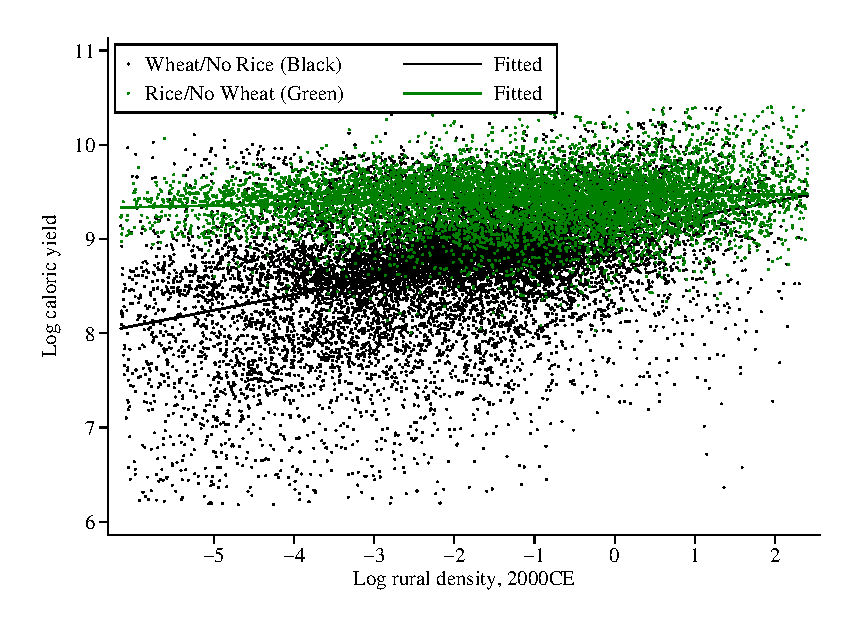
\includegraphics[width=.8\textwidth]{fig_beta_crop.eps}
\end{center}
\end{frame}

\begin{frame}{Results by Crop}
\begin{center}
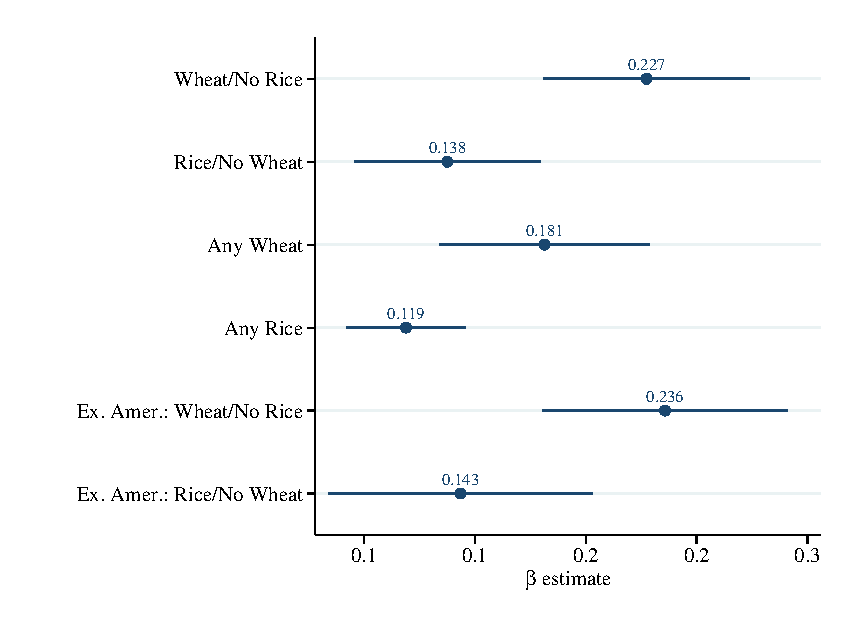
\includegraphics[width=.8\textwidth]{fig_coef_crop.eps}
\end{center}
\end{frame}

\begin{frame}{Results by Crop}

{\scriptsize
\begin{tabularx}{\textwidth}{lXXXXXX}
\midrule
\multicolumn{7}{l}{Dependent Variable in all panels: Log caloric yield ($A_{isc}$)} \\ \\
\multicolumn{7}{l}{Panel A: Wheat and rice} \\
 & \multicolumn{6}{c}{Inclusion by crop suitability:} \\ \cmidrule(lr){2-7}
 & \multicolumn{4}{c}{Entire world:} & \multicolumn{2}{c}{Ex. Americas:}\\ \cmidrule(lr){2-5} \cmidrule(lr){6-7} 
 & Wheat$>$0& Wheat=0 &         &        & Wheat$>$0   & Wheat=0   \\
 & Rice=0 & Rice$>$0  & Wheat$>$0 & Rice$>$0 & Rice=0    & Rice$>$0   \\
 & (1) & (2) & (3) & (4) & (5) & (6) \\
\midrule
rurd_reg            &       0.227&       0.138\\
                    &     (0.024)&     (0.021)\\
\midrule
p-value $\beta=0$   &       0.000&       0.000\\
p-value $\beta=\beta^{Wheat}$&            &    .0049448\\
Countries           &         106&          74\\
Observations        &    12627.00&    20423.00\\
Adjusted R-square   &        0.21&        0.19\\

\midrule
\end{tabularx}
}
\end{frame}

\begin{frame}{Results by Crop}

{\scriptsize
\begin{tabularx}{\textwidth}{lXXXXXX}
\midrule
\multicolumn{7}{l}{Dependent Variable in all panels: Log caloric yield ($A_{isc}$)} \\ \\
\multicolumn{7}{l}{Panel B: Tropical crops} \\
                   & \multicolumn{6}{c}{Inclusion is wheat suitability = 0, but:} \\ \cmidrule(lr){2-7}
                   &            &              &          &   Pearl       &  Sweet      & \\
& Cassava$>$0 & Cowpea$>$0  & Maize$>$0 & Millet$>$0 & Potato$>$0 & Yams$>$0   \\
\midrule
Log rural density   &       0.140&       0.144&       0.143&       0.154&       0.144&       0.140\\
                    &     (0.021)&     (0.020)&     (0.020)&     (0.019)&     (0.020)&     (0.020)\\
\midrule
p-value $\beta=0$   &       0.000&       0.000&       0.000&       0.000&       0.000&       0.000\\
Countries           &          74&          80&          78&          72&          77&          78\\
Observations        &        8052&        8312&        8377&        6590&        8354&        8269\\
Adjusted R-square   &        0.13&        0.13&        0.13&        0.13&        0.13&        0.12\\

\midrule
\end{tabularx}
}

\end{frame}

\begin{frame}{Results by Crop}

{\scriptsize
\begin{tabularx}{\textwidth}{lXXXXXX}
\midrule
\multicolumn{7}{l}{Dependent Variable in all panels: Log caloric yield ($A_{isc}$)} \\ \\
\multicolumn{7}{l}{Panel C: Temperate crops} \\
                   & \multicolumn{6}{c}{Inclusion is rice suitability = 0, but:} \\ \cmidrule(lr){2-7}
                   &            & Buck-        &          &          &         & White \\
                   & Barley$>$0 & wheat$>$0  & Oats$>$0 & Flax$>$0 & Rye$>$0 & Potato$>$0   \\
\midrule
Log rural density   &       0.227&       0.228&       0.234&       0.228&       0.235&       0.227\\
                    &     (0.024)&     (0.025)&     (0.025)&     (0.025)&     (0.025)&     (0.023)\\
\midrule
p-value $\beta=0$   &       0.000&       0.000&       0.000&       0.000&       0.000&       0.000\\
Countries           &         106&          76&          72&          74&          72&         105\\
Observations        &       12627&       11162&       11089&       11035&       11106&       12494\\
Adjusted R-square   &        0.21&        0.23&        0.23&        0.23&        0.23&        0.22\\

\midrule
\end{tabularx}
}
\end{frame}

\begin{frame}{Results by Climate Zone}

\end{frame}


\begin{frame}{Results by Climate Zone}
\begin{center}
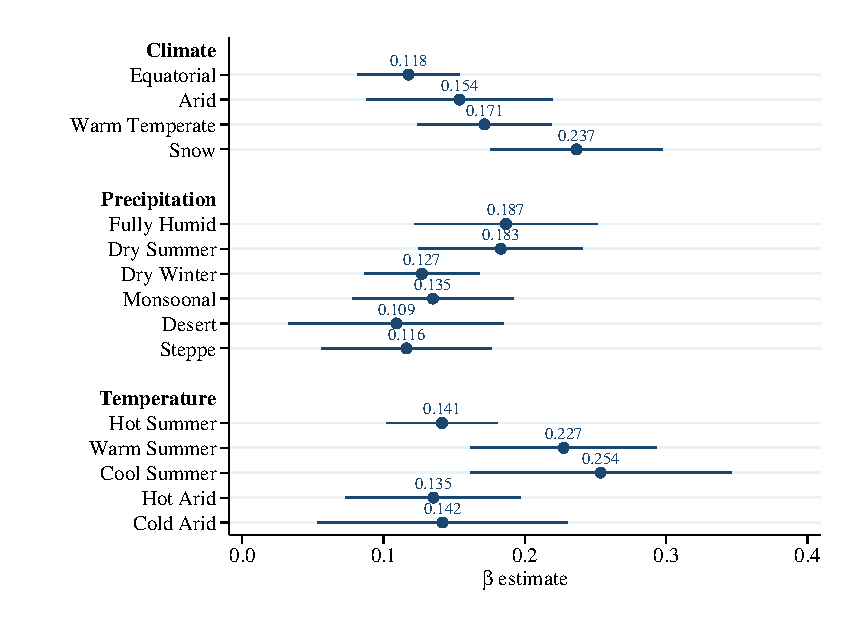
\includegraphics[width=.8\textwidth]{fig_coef_kg.eps}
\end{center}
\end{frame}

\begin{frame}{Robustness}\label{robustness}
``Robust'' meaning
\begin{itemize}
  \item Absolute and relative size of $\beta$ estimates across samples are similar
  \item Hypothesis tests return similar results
\end{itemize}
Robustness checks:
\begin{itemize}
  \item Use province level data (with country FE) \hyperlink{regprov}{\beamerbutton{Results}}
  \item Use rural density from 1900 from HYDE \hyperlink{reg1900}{\beamerbutton{Results}}
  \item Use untrimmed samples of rural density and/or agricultural productivity
  \item Use districts with fewer than 100 rural residents
  \item Clustered standard errors (at province level)
\end{itemize}
\end{frame}

\begin{frame}{Measurement Error}
Measurement error in rural density data
\begin{itemize}
  \item Creates attentuation bias
  \item Is measurement error more pronounced in some regions (e.g. SE Asia) and driving results?
  \item True variance of $\ln L_{Aisc}/X_{isc}$ would have to be one-third of measured variance
  \item Implies one-third of districts have rural density mis-stated by factor of $>2$ or $<0.5$
\end{itemize}
\end{frame}

\begin{frame}{Measurement Error}
Measurement error of land area, $X_{isc}$, specifically
\begin{itemize}
  \item We are using total land area, not agricultural area, so $X_{isc}$ always overstated
  \item Systematic mismeasurement of districts within a province not a problem
  \item Variation in systematic mismeasurement across provinces not a problem (FE)
  \item Problem is \textit{variation in variation of mismeasurement} across provinces
  \item Some provinces have more geographic variation across districts?
  \item Provinces with low $\beta$ estimates do not have higher variance of geographic characteristics
\end{itemize}
\end{frame}

\begin{frame}{Mobility of Workers?}
Mobility of workers across districts within a province?
\begin{itemize}
  \item<1-> If workers immobile, may create similar densities across districts
  \item<1-> Estimated $\beta$ would be falsely high?
  \item<1-> Would have to be that frictions more prevalent in high-$\beta$ places (e.g. Europe or N. Africa)
  \item<2-> Or, workers immobile, but demographic behavior varies widely by district?
  \item<2-> Estimated $\beta$ would be falsely low? 
  \item<2-> Would have to be demography is more variable in low-$\beta$ places (e.g. Sub-Saharan Africa)
\end{itemize}
\end{frame}

\begin{frame}{Elasticity of Substitution?}\label{eos}
What if land and labor do not have elasticity of subs. equal to one?
\begin{itemize}
  \item Elasticity of output w.r.t. land depends on rural density $L_A/X$
  \item With EOS more than one, higher density, lower elasticity
  \item Do results fit this?
  \begin{itemize}
    \item South/SE Asia, some SS Afr are high density, low $\beta$
    \item ..but C/S America, other SS Afr are low density, low $\beta$
    \item ..but N America lowest density, not highest $\beta$
  \end{itemize}
\end{itemize}
\hfill \hyperlink{rurdbeta}{\beamerbutton{Density?}}
\end{frame}


\section{Implications}

\begin{frame}{Back to the model}
If each person consumes $c_A$ in agric. goods, with $L$ people, then:
\begin{equation}
c_A L = \sum_{i \in I} A_{i} X_{i}^{\beta} \left(K_{Ai}^{\alpha}L_{Ai}^{1-\alpha}\right)^{1-\beta}, \label{EQ_caL}
\end{equation}
Assume that capital and labor are mobile between districts within region $I$, but also between agric. and non-agric. Can solve for
\begin{equation}
\frac{L_{A}}{L} = \left(\frac{c_A L^{\beta}}{(K/L)^{\alpha(1-\beta)} \left(\sum_{i \in I} A_i^{1/\beta} X_i\right)^{\beta}} \right)^{1/(1-\beta)} \label{EQ_LaL}
\end{equation}
where $K/L$ is aggregate capital/labor ratio.
\end{frame}

\begin{frame}{Real Wage}
With labor mobile between agric. and non-agric., then 
\begin{equation}
    p_N w_N = p_A w_A
\end{equation}
where $p_j$ is nominal price of good $j$, and $w_j$ is wage in terms of output in $j$. Combine with $w_A = \phi_L Y_A/L_A$ definition from before to get
\begin{equation}
    \frac{p_N w_N}{p_A} = \frac{\phi_L c_A}{L_A/L}. \label{EQ_realwage}
\end{equation}
This is a ``grain wage''. Non-agricultural nominal wage deflated by the price of agricultural goods. 
\end{frame}

\begin{frame}{Elasticities}
With respect to population shocks
\begin{itemize}
  \item $\frac{\partial L_A/L}{\partial L}\frac{L}{L_A/L} = \frac{\beta}{1-\beta}$
  \item $\frac{\partial p_Nw_N/p_A}{\partial L}\frac{L}{p_Nw_N/p_A} = -\frac{\beta}{1-\beta}$
\end{itemize}
With respect to productivity shocks in agric. (equal across all districts)
\begin{itemize}
  \item $\frac{\partial L_A/L}{\partial A}\frac{A}{L_A/L} = \frac{1}{1-\beta}$
  \item $\frac{\partial p_Nw_N/p_A}{\partial A}\frac{A}{p_Nw_N/p_A} = -\frac{1}{1-\beta}$
\end{itemize}
\end{frame}

\begin{frame}{A Toy Calibration}
Set up three economies, each with
\begin{itemize}
  \item $L = 1$
  \item $A = 1$
  \item $X = 1$
\end{itemize}
but where the value of $\beta$ takes on values (0.05, 0.15, 0.25). Initial value of $c_A$ is set so that $L_A/L = 0.85$ in each.

\vspace{.2cm} Look at effect of variation in $L$ and $A$ on 
\begin{itemize}
  \item $L_A/L$
  \item Real wage
\end{itemize}

\end{frame}

\begin{frame}{A Toy Calibration}
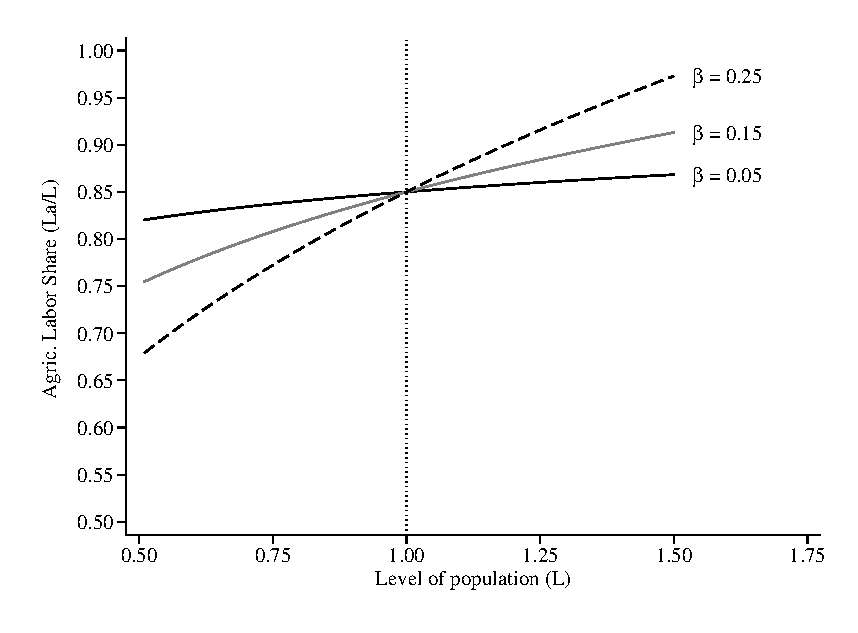
\includegraphics[width=.8\textwidth]{fig_sim_L_LaL.eps}
\end{frame}

\begin{frame}{A Toy Calibration}
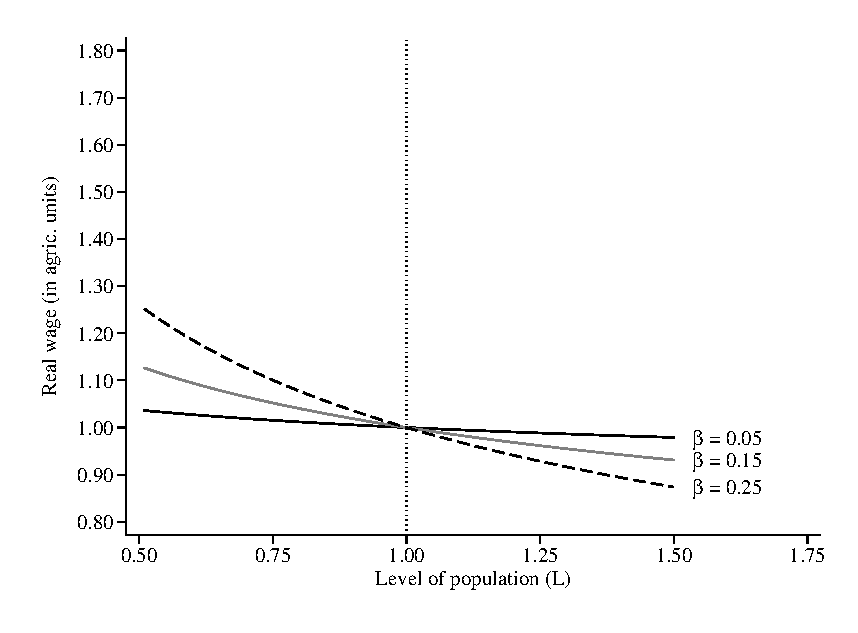
\includegraphics[width=.8\textwidth]{fig_sim_L_w.eps}
\end{frame}

\begin{frame}{A Toy Calibration}
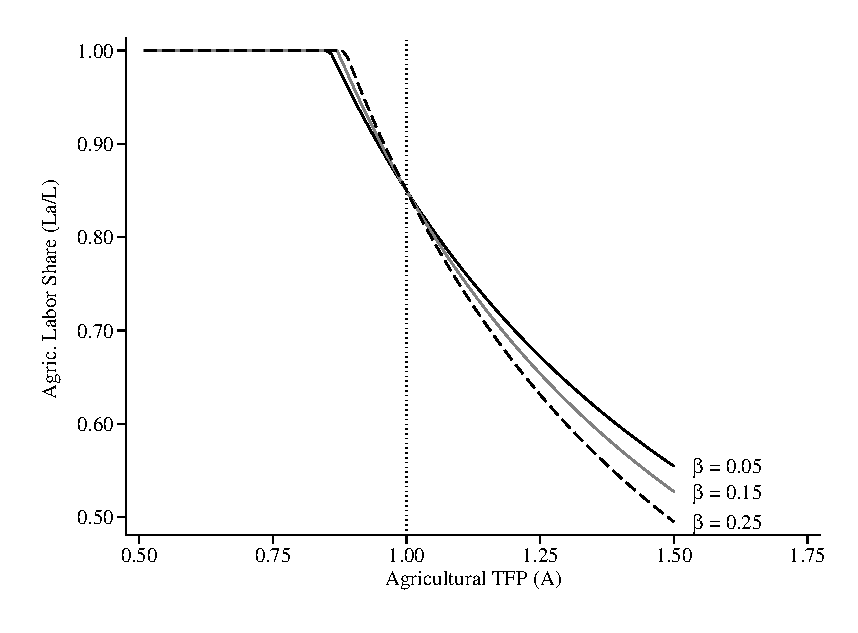
\includegraphics[width=.8\textwidth]{fig_sim_A_LaL.eps}
\end{frame}

\begin{frame}{A Toy Calibration}
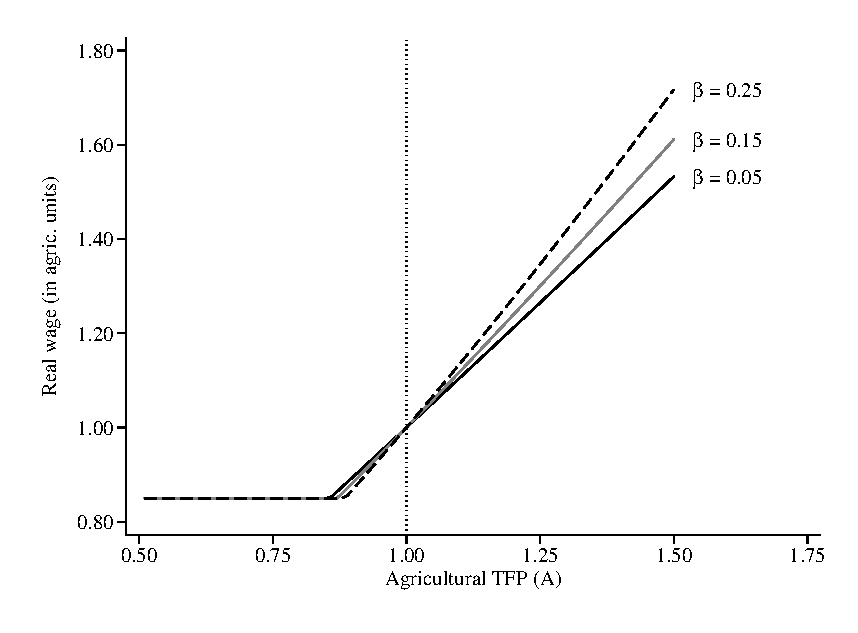
\includegraphics[width=.8\textwidth]{fig_sim_A_w.eps}
\end{frame}

\section{Conclusion}

\begin{frame}{Conclusion}
\begin{itemize}
  \item Define the Malthusian constraint as the elasticity of output w.r.t. land
  \item Estimate constraint from variation in rural density within provinces
  \item Constraint is ``tight'' (0.20-0.30) in temperate areas (N. China, Europe, US/Canada, S. Africa)
  \item Constraint is ``loose'' (0.05-0.10) in tropical areas (S. China, SE Asia, C. Africa, S/C America)
  \item Constraint dictates the sensitivity of $L_A/L$ and real wage to population and productivity
\end{itemize}
\end{frame}

\section{Appendix Slides}

\begin{frame}{A Toy Model}\label{toy}
Single sector production with produtivity, $A$, fixed factor, $X$, and labor, $L$. 
\begin{equation}
Y = A X^\beta L^{1-\beta}
\end{equation}
Average product of labor is:
\begin{equation}
    \frac{Y}{L} = A \left(\frac{X}{L}\right)^{\beta}.
\end{equation}
Elasticity of average product with respect to $L$ depends on $\beta$.
\end{frame}

\begin{frame}{A Toy Model}
Assume population process works such that average product is always $c$, density is
\begin{equation}
    \frac{L}{X} = \left(\frac{A}{c}\right)^{1/\beta}.
\end{equation}

\begin{itemize}
  \item Density does not tell us whether land constraint is tight or loose 
  \item But $\beta$ tells us how sensitive density is to productivity
\end{itemize}
\hfill \hyperlink{define}{\beamerbutton{Return}}
\end{frame}

\begin{frame}{Interaction Regression}\label{interaction}
Combine a given sample with the reference sample (denoted by $Ref$). Run the following regression with interaction terms
\begin{eqnarray}
    \ln A_{isc} = \beta \ln L_{Aisc}/X_{isc} + (\beta^{Ref} - \beta) \ln L_{Aisc}/X_{isc} \times I(Ref) \\ \nonumber
    + \gamma_{sc} + \delta' \mathbf{Z}_{isc} + (\delta^{Ref} - \delta)'\mathbf{Z}_{isc} \times I(Ref) + \epsilon_{isc}. \label{EQ_interaction}
\end{eqnarray}
where $I(Ref)$ is an indicator for the reference region. Our hypothesis test is $H_0: \beta^{Ref} - \beta = 0$, the coefficient on the interaction term for rural density. 

\hfill \hyperlink{testing}{\beamerbutton{Return}}
\end{frame}


\begin{frame}{Results by Major Region, 1900 CE}\label{reg1900}

{\scriptsize
\begin{tabularx}{\textwidth}{lXXXXXX}
\midrule
\multicolumn{7}{l}{Dependent Variable: Log caloric yield ($A_{isc}$)} \\
 & \multicolumn{6}{c}{Region:} \\ \cmidrule{2-7}
 &        & East \& & Sub-        & North     & South \&  &  \\
 &        & South   & Saharan     & Africa \& & Central   & U.S. and \\
 & Europe & Asia    & Africa      & West Asia & America   & Canada \\
 & (1) & (2) & (3) & (4) & (5) & (6) \\
\midrule
Log rural density   &       0.413&       0.254&       0.061&       0.269&       0.070&       0.316\\
                    &     (0.046)&     (0.054)&     (0.032)&     (0.035)&     (0.029)&     (0.064)\\
\midrule
p-value $\beta=0$   &       0.000&       0.000&       0.054&       0.000&       0.016&       0.000\\
p-value $\beta=\beta^{Eur}$&           .&       0.025&       0.000&       0.013&       0.000&       0.217\\
Countries           &          34&          24&          43&          18&          25&           2\\
Observations        &        7514&        6761&        3210&        2762&        9131&        2782\\
Adjusted R-square   &        0.43&        0.34&        0.31&        0.37&        0.24&        0.40\\

\midrule
\end{tabularx}
}

\hfill \hyperlink{robustness}{\beamerbutton{Return}}
\end{frame}

\begin{frame}{Results by Sub-Region, 1900 CE}

{\scriptsize
\begin{tabularx}{\textwidth}{lXXXXX}
\midrule
\multicolumn{6}{l}{Dependent Variable in both panels: Log caloric yield ($A_{isc}$)} \\ \\
\\
Panel A & \multicolumn{5}{c}{Sub-Region:} \\ \cmidrule{2-6}
 &          &         &             &  \multicolumn{2}{c}{Excl. China} \\ \cmidrule(lr){5-6}
 & North \& &         &              & South \&  & Central \&             \\
 & Western  & Eastern & Southern     & Southeast & West        \\
 & Europe   & Europe  & Europe       & Asia      & Asia      \\
 & (1) & (2) & (3) & (4) & (5) \\
\midrule
Log rural density   &       0.363&       0.414&       0.291&       0.090&       0.264\\
                    &     (0.055)&     (0.027)&     (0.025)&     (0.035)&     (0.062)\\
\midrule
p-value $\beta=0$   &       0.000&       0.000&       0.000&       0.010&       0.000\\
p-value $\beta=\beta^{NWEur}$&           .&       0.247&       0.323&       0.000&       0.232\\
Countries           &          16&           9&           9&          13&          18\\
Observations        &        1628&        4772&        1114&        3921&        2762\\
Adjusted R-square   &        0.35&        0.45&        0.31&        0.24&        0.26\\

\midrule
\end{tabularx}
}

\hfill \hyperlink{robustness}{\beamerbutton{Return}}
\end{frame}

\begin{frame}{Results by Sub-Region, 1900 CE}

{\scriptsize
\begin{tabularx}{\textwidth}{lXXXXX}
\midrule
\multicolumn{6}{l}{Dependent Variable in both panels: Log caloric yield ($A_{isc}$)} \\ \\
\\
Panel B & \multicolumn{5}{c}{Sub-Region:} \\ \cmidrule{2-6}
 &           &   &           &          &             \\
 & Temperate & Tropical  & Tropical & South    & North    \\
 & Americas  & Americas  & Africa   & Africa   & Africa     \\
\midrule
Log rural density   &       0.200&       0.080&       0.049&       0.257&       0.296\\
                    &     (0.059)&     (0.028)&     (0.033)&     (0.091)&     (0.041)\\
\midrule
p-value $\beta=0$   &       0.001&       0.004&       0.130&       0.005&       0.000\\
p-value $\beta=\beta^{NWEur}$&       0.042&       0.000&       0.000&       0.316&       0.322\\
Countries           &           5&          22&          39&           4&           5\\
Observations        &        3183&        8730&        3032&         178&        1147\\
Adjusted R-square   &        0.22&        0.12&        0.16&        0.34&        0.30\\

\midrule
\end{tabularx}
}

\hfill \hyperlink{robustness}{\beamerbutton{Return}}
\end{frame}

\begin{frame}{Results by Major Region, 2000 CE, Provinces}\label{regprov}

{\scriptsize
\begin{tabularx}{\textwidth}{lXXXXXX}
\midrule
\multicolumn{7}{l}{Dependent Variable: Log caloric yield ($A_{isc}$)} \\
 & \multicolumn{6}{c}{Region:} \\ \cmidrule{2-7}
 &        & East \& & Sub-        & North     & South \&  &  \\
 &        & South   & Saharan     & Africa \& & Central   & U.S. and \\
 & Europe & Asia    & Africa      & West Asia & America   & Canada \\
 & (1) & (2) & (3) & (4) & (5) & (6) \\
\midrule
Log rural density   &       0.385&       0.267&       0.124&       0.382&       0.027&       0.111\\
                    &     (0.101)&     (0.092)&     (0.044)&     (0.112)&     (0.068)&     (0.280)\\
\midrule
p-value $\beta=0$   &       0.000&       0.004&       0.005&       0.001&       0.697&       0.693\\
p-value $\beta=\beta^{Eur}$&           .&       0.389&       0.018&       0.983&       0.003&       0.358\\
Countries           &          34&          23&          43&          18&          23&           2\\
Observations        &         507&         570&         525&         282&         355&          47\\
Adjusted R-square   &        0.16&        0.19&        0.13&        0.19&        0.08&        0.13\\

\midrule
\end{tabularx}
}

\hfill \hyperlink{robustness}{\beamerbutton{Return}}
\end{frame}

\begin{frame}{Results by Sub-Region, 2000 CE, Provinces}

{\scriptsize
\begin{tabularx}{\textwidth}{lXXXXX}
\midrule
\multicolumn{6}{l}{Dependent Variable in both panels: Log caloric yield ($A_{isc}$)} \\ \\
\\
Panel A & \multicolumn{5}{c}{Sub-Region:} \\ \cmidrule{2-6}
 &          &         &             &  \multicolumn{2}{c}{Excl. China} \\ \cmidrule(lr){5-6}
 & North \& &         &              & South \&  & Central \&             \\
 & Western  & Eastern & Southern     & Southeast & West        \\
 & Europe   & Europe  & Europe       & Asia      & Asia      \\
 & (1) & (2) & (3) & (4) & (5) \\
\midrule
Log rural density   &       0.662&       0.343&       0.169&       0.044&       0.384\\
                    &     (0.114)&     (0.074)&     (0.102)&     (0.016)&     (0.069)\\
\midrule
p-value $\beta=0$   &       0.000&       0.000&       0.099&       0.007&       0.000\\
p-value $\beta=\beta^{NWEur}$&           .&       0.006&       0.004&       0.000&       0.037\\
Countries           &          16&           9&           9&          13&          18\\
Observations        &         166&         206&         135&         370&         303\\
Adjusted R-square   &        0.20&        0.24&        0.15&        0.17&        0.24\\

\midrule
\end{tabularx}
}

\hfill \hyperlink{robustness}{\beamerbutton{Return}}
\end{frame}

\begin{frame}{Results by Sub-Region, 2000 CE, Provinces}

{\scriptsize
\begin{tabularx}{\textwidth}{lXXXXX}
\midrule
\multicolumn{6}{l}{Dependent Variable in both panels: Log caloric yield ($A_{isc}$)} \\ \\
\\
Panel B & \multicolumn{5}{c}{Sub-Region:} \\ \cmidrule{2-6}
 &           &   &           &          &             \\
 & Temperate & Tropical  & Tropical & South    & North    \\
 & Americas  & Americas  & Africa   & Africa   & Africa     \\
\midrule
Log rural density   &       0.162&       0.014&       0.115&       0.406&       0.621\\
                    &     (0.122)&     (0.070)&     (0.044)&     (0.224)&     (0.133)\\
\midrule
p-value $\beta=0$   &       0.188&       0.839&       0.009&       0.071&       0.000\\
p-value $\beta=\beta^{NWEur}$&       0.003&       0.000&       0.000&       0.310&       0.818\\
Countries           &           5&          20&          39&           4&           5\\
Observations        &          85&         317&         497&          28&          88\\
Adjusted R-square   &        0.14&        0.08&        0.13&        0.21&        0.28\\

\midrule
\end{tabularx}
}

\hfill \hyperlink{robustness}{\beamerbutton{Return}}
\end{frame}

\begin{frame}{Relationship fo $\beta$ to rural density, by province}\label{rurdbeta}
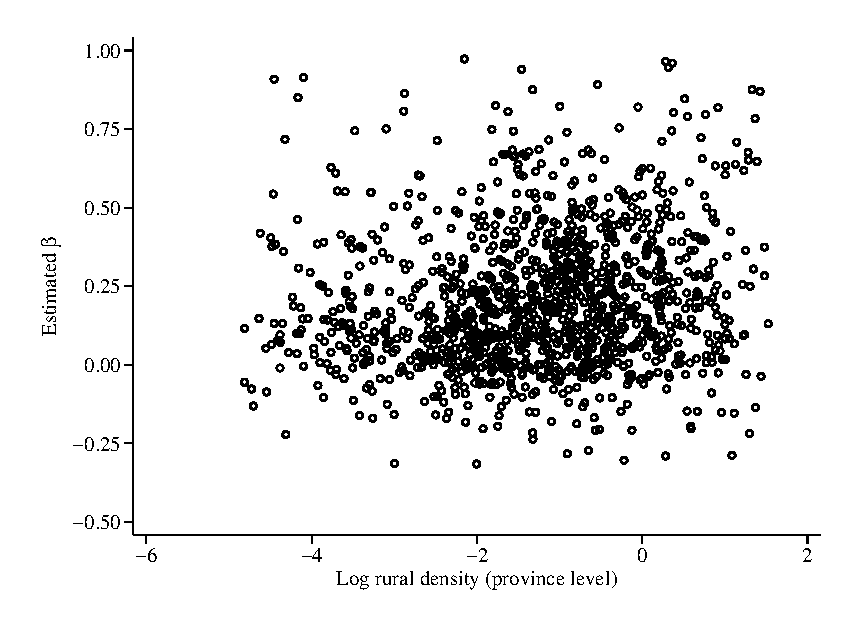
\includegraphics[width=.8\textwidth]{fig_beta_rurd.eps}
\hfill \hyperlink{eos}{\beamerbutton{Return}}
\end{frame}

\end{document}
